\documentclass[10pt]{article}
\usepackage[cm]{fullpage}
\usepackage{graphicx}
\begin{document}

\title{Software Engineering (Practice) Coursework 1 \\ Estimation and Planning}
\author{Group 2 (Thomas Burnell, Andrei Cioara, Jeremy Kong, Andrea Michi, Alice Sibold)}
\maketitle

\section{Background}
Individuals often face the problem of having to develop an itinerary for efficiently completing various tasks, many of which can only be done at certain locations. For example, they may have to withdraw cash and meet a friend for coffee during their (short) lunch break. Such an itinerary may be easily planned by one who knows the exact locations he needs to visit, the order in which he should visit them, and their distances from each other / his current position, however triviality vanishes when any of these are unknown. Our project aims to provide a user with a system that can determine a suitable route to complete all of his tasks. This differs from existing routing products in that our system is intended to be able to cope with planning routes incorporating multiple destinations in an arbitrary order, as well as situations where the exact locations or even types of locations may not necessarily be well-defined. In motivation, consider a user who wants to post a letter and fetch a coffee. Our application could suggest visiting a postbox the user is unaware of in a street closely neighbouring a nearby Starbucks store, rather than venturing to the Post Office he is familiar with, situated farther away.

\section{Identifying Customer Requirements}
\subsection{Customer Requirements}
This project was mooted by the Project Supervisor (PS) Prof. Sophia Drossoupoulou as a customer. Our product appears to have a large potential user-base; in our experience we have found that it is fairly common for students and professionals alike to need to complete multiple tasks under time constraints. This could prove advantageous, as we would have ready access to customers and thus be able to easily identify users' priorities and key requirements.\\\\
In order to gather requirements and move closer to a more well-defined project specification, we held a meeting with the PS, as well as other brainstorming sessions as a group. Together with the PS, we initially identified two different routing problems that might be both useful and applicable to solve:
\begin{itemize}
\item Given a list of tasks and their possible locations, find a route that goes through some of the locations, at a minimum cost, such that all tasks are completed - this is an instance of the Generalised Travelling Salesman Problem (GTSP); it can be reduced to the standard TSP\footnote{Arash Behzad, Mohammad Modarres (2002). ``A New Efficient Transformation of Generalised Traveling Salesman Problem into Traveling Salesman Problem".}. While both problems are NP-hard, exponential-time algorithms have solved instances of the problem on the order of $10^5$ nodes\footnote{Applegate, D. L.; Bixby, R. M.; Chvátal, V.; Cook, W. J. (2006), ``The Traveling Salesman Problem", ISBN 0-691-12993-2.}.
\item Finding a point satisfying constraints on routes to other destinations - this could be solved using stochastic hill-climbing algorithms, or expanding graphs of points reachable from said other destinations within the provided constraints and finding their intersection.
\end{itemize}
When considering the two alternatives we aimed for maximum customer satisfaction; we found difficulty in finding sufficiently many use-cases as well as readily accessible customers for the second option and thus opted for the first. \\\\
In this project, we intend to work closely with the PS, as well as source feedback from other students. As discussed later in section 4.2.4, we will hold frequent demo meetings with the PS, where any feedback gathered will help us to tailor our plans for subsequent iterations accordingly. Based on our meetings with our PS as well as internal discussions within the team, the key requirements for our project are as follows:
\begin{enumerate}
\item Users should be able to specify one or more tasks (from a pre-defined selection) that they need to complete. (These tasks may or may not have user-defined locations.)
\item Users should be able to enter information about these tasks through a web UI.
\item Users should be able to have their tasks mapped to locations where they might be completed.
\item Users should be able to indicate a location from which they begin travelling to possible locations.
\item Users should be given an \textit{optimal} or close to optimal route that incorporates locations such that the user can complete all of his or her tasks. 
\item Users should be presented the output of our algorithm through a web UI.
\item Users should have the output visualised graphically; the PS suggested using the Google Maps API for visualisation.
\end{enumerate}
In addition to the requirements outlined above, we also gathered ideas for stretch goals. Should we have the time, we would like to implement the following:
\begin{enumerate}
\item Users should be able to use our application on their mobile devices, by interacting with a mobile-friendly UI.
\item Users should be able to integrate this system with mobile personal assistants, such as Google Now.
\item Users should have the possibility of choosing different criteria for routes (such as minimising travel time, using scenic routes, or minimising travel expenditure).
\end{enumerate}

\subsection{Release Plan}
With this in mind, our team created an initial release plan. The plan describes which customer requirements we are likely to work on during each iteration (at a high level); we will decompose these requirements to finer-grained tasks at the beginning of each iteration. This plan is still highly tentative, as customer requirements might change, and also because we currently do not have a clear estimate of our team's velocity. We estimated the relative engineering scope of the requirements, and assigned requirements to iterations accordingly - bearing in mind dependencies between requirements as well as the ability (or inability) to present something visible to the customer at the end of each iteration.
\begin{center}
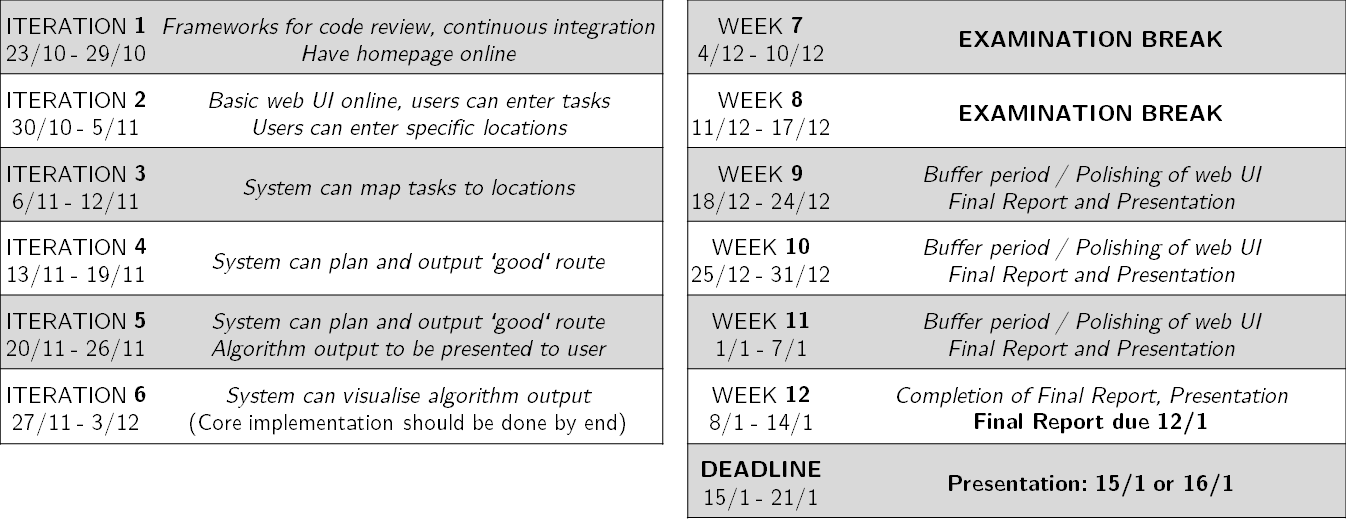
\includegraphics[scale=0.75]{release_plan.png}
\end{center}
\section{Modularity of Product Design}
We identified fairly early on that the architecture of our application can be designed such that it is composed of three distinct components: \begin{enumerate}
\item \textbf{Web interface} $-$ our application will present a rich web UI to the user.
\item \textbf{Mapping from tasks to locations} $-$ our application will need to determine a set of points where a user may carry out (a) specified task(s).
\item \textbf{Routing through locations} $-$ our application will then need to calculate the best route a user can take to carry out his tasks, based on the known points from component 2.
\end{enumerate}
This is best illustrated through a diagram -- consider Figure 1 in the appendix.\\\\
As learned through Software Engineering courses and real-life experience, a modular design will help to reduce the rigidity, fragility and immobility of our code. As explained later in section 4.2, we will complete our project by working through lots of small, well-defined tasks. We aim to define such tasks in a way that they relate to -- more often than not -- just one of the components above. For example, we will define tasks such as ``Display route returned by API call on a Google map" and ``Calculate route using GTSP using a set of given points", rather than ``Calculate and display a route on a Google map". \textit{(The tasks used in example here are designed for clarity; clearly in practice, these tasks would be further decomposed.)} \\\\
In addition, a modular design allows for a greater scope of extension. Separating out concerns into distinct interacting components will allow us to introduce additional functionality and features later down the line, much easier than if we were working in one monolithic codebase. For example, it has been suggested that a stretch goal for our application may be to allow for integration with mobile personal assistants such as Google Now, and/or Cortana. Such a feature could be implemented by introducing another component to our system (perhaps ``Assistant Integrator"), without the need to make any significant code changes in other parts of the system.

\section{Agile Methodologies}
\subsection{Overview}
In an age where consumers are becoming increasingly dependent on technology to solve many of life's (ever evolving) problems, it is vital that technology firms work in ways which allow them to be responsive to new and changing requirements. As a team working to design and build a product to a customer's specification, we identify a need to work in similar ways. Furthermore, as a team of full-time students with a very limited timescale, we see it of paramount importance to be able to work responsively, remaining flexible to allow for the inevitable maturation of our initially vague project brief.\\\\
Several members of our team have past experience with Agile and/or iterative development, largely through the course of summer internships and placements. In particular, we appreciated the merit of iteratively releasing our work; this allowed us to both refine our product to better meet the requirements of our customers (or managers in certain cases), as well as better gauge the scope of what we could do given a tightly-defined deadline.\\\\
Our team discussed several possible project and/or engineering management practices from various Agile development approaches (such as Scrum, Extreme Programming (XP) and Kanban), and considered their suitability bearing in mind our team's specific needs.\\\\
We found that not all of these industry `best practices' as written are suitable for our team -- to some extent, this is because we are currently students (and not software engineers in industry). We have to attend potentially up to 8 hours of lectures per day, and complete other coursework and assignments in parallel with this project. Thus, for example, daily standup meetings would not be practical since we might not necessarily be able to work on the project everyday. Furthermore, our team has a very full aggregate timetable; as a result, the time we can meet as a team is severely constrained as well. Consequently, many of these `best practices' need to be adapted or modified to make them suitable for our working style.\\\\
During a summer internship, one team member gained exposure to Kanban processes. Working in a team which took such approaches to development, he was able to identify some of the ways in which they work well, but also how they could fail when applied to certain types of work. It was observed that, when working on operational tasks (such as bug fixing, small feature enhancements, etc.), limiting the number of tasks in progress and maintaining a prioritised backlog worked well; working in this way allowed for a continuous flow at a high velocity. During the placement the team switched to working on a larger 3-month project, where they were building an entirely new system from the ground up. Not changing the choice of Agile methodologies (for example switching to Scrum) soon proved to be problematic. With a new large project came many unknowns, and the lack of scheduled planning meetings and customer demonstrations soon resulted in a number of completed tasks needing respecification and thus reimplementation, leaving the team unable to push out new features at the rate at which they were able to when working operationally. As a team also working on an entirely new product, we feel that Kanban is too loose, and favour methodologies where planning meetings, demonstrations and timeboxed iteration periods are of high importance.\\\\
After much deliberation, we decided to adopt several project management practices from Scrum, as well as some of the engineering processes from XP. These practices, and our motivations for adopting them, will be discussed in the following sections.

\subsection{Project Management Practices: Scrum}
\subsubsection{Overview}
Our team were unanimous in the belief that the approach we take to project management will have huge influence on our success. Working with a fairly large team (compared to projects of previous years) and a limited timescale to produce a rather large product, we realised that without placing an importance on the management of our work/team but simply the engineering practices we adopt, we would risk a slow velocity and thus potentially not completing an application which satisfies all of our customer's requirements.\\\\
We decided to adopt some of the practices of Scrum to manage how we work. We appreciate how well Scrum can work in industry among teams of software engineers, Business Analysts and managers, however we have chosen to adapt some principles somewhat to better suit our (busy, student) team.\\\\
Some of the team have experience in working with Scrum through summer internships, and were thus able to share their views on what practices may/may not work for us. This, along with material learnt through the Software Engineering (Practice) course and additional research carried out online brought us to a position where we felt confident making the choices we will now outline.

\subsubsection{Sprints}
We are working through 1-week Sprint cycles. Typically in industry such cycles last between 2 and 4 weeks\footnote{\texttt{https://stefanroock.wordpress.com/2012/12/20/shades-of-scrum-Sprint-length/}}, however with a timescale of only 6 weeks to complete the core implementation of our project, we identified that this would leave us having only 3 iterations and so less opportunity for feedback/requirement adaptation\footnote{\texttt{http://agilepainrelief.com/notesfromatooluser/2013/07/choosing-Sprint-length-shorter-trumps-longer.html}} -- a poor granularity. Also, short cycles will help us to make more accurate velocity predictions.\\\\
We hold Sprint planning meetings at the beginning of each cycle, where we analyse and break down high-level stories from the top of our prioritised (Product) ``Backlog". Though the PS is acting as our customer/product owner, she will not be in attendance at these meetings due to her busy academic schedule, however all members of our team will be present. All tasks we decide to commit to the upcoming Sprint are then placed in the ``To-Do" (Sprint Backlog) column on our storyboard (see section 5 for details). As is traditional, we approach the Product Backlog in a strict priority fashion\footnote{\texttt{http://www.mountaingoatsoftware.com/agile/scrum/product-backlog}}. However, we also approach our Sprint Backlog in a similar way. We learnt that Scrum teams typically allow for more freedom as to the ordering of task completion mid-Sprint\footnote{\texttt{https://www.scrumalliance.org/community/articles/2009/december/scrum-in-a-nutshell}; see section on `The Sprint'}, however in preparation for the possibility of not completing all tasks in a Sprint we chose to encourage -- where reasonable -- a somewhat stricter approach, to guarantee the completion only of the highest priority tasks.
\subsubsection{Velocity Measurement}
We will use velocity measurement as a way of planning realistic and achievable Sprints. Each task will be given a point score after estimation, and the number of points of tasks completed from one Sprint will help us to more accurately predict how many pointed tasks should be included in the next.

\subsubsection{Demonstrations}
We meet with the PS for one hour each Thursday at 11am. We will be using this time to showcase our latest work, and gather as much feedback as possible. In addition, we will discuss the upcoming Sprint so that any features that the PS feels are of higher priority are brought to the top of our (Product) ``Backlog", ready for the subsequent Sprint planning meeting.

\subsubsection{Retrospectives}
We will hold short retrospectives after each Sprint to discuss our team work and assess how well our practices are working. As we are currently in our first Sprint, we have not yet held a retrospective. Since our Sprints are relatively short, we aim to be able to complete this in 10-15 minutes before we begin to plan the following Sprint. We struggle to find any more time in our aggregate timetable to allow for a longer meeting, however we feel that this short time is sufficient.

\subsubsection{Scrum Master}
We chose to elect Tom as the Scrum Master (SM) to act as team lead. Unlike traditional Scrum however, due to the nature of our team the SM will also serve as a developer. Our SM has the following three responsibilities\footnote{\texttt{http://www.mountaingoatsoftware.com/agile/scrum/scrummaster}}, additional to his development roles:
\begin{enumerate}
\item Remove impediments that are obstructing the team's work. For example, if the team require additional resources or support with any tasks, the SM will identify what can be done to resume progress.
\item Own the success of the team's progress. This involves ensuring all deadlines are met and planned for accordingly, as well as making sure that the highest priority tasks as identified with the PS are planned for in the next Sprint. Additionally, the SM will pay close attention to the progression of each task mid-Sprint, and identify any bottlenecks. Frequent communication within the team will be encouraged by the SM.
\item Provide a point of communication between all parties. The SM will own all communication between the team and the PS, for example if additional meetings need to be scheduled.
\end{enumerate}

\subsubsection{Scrum vs. XP}
We considered project management practices from Scrum and XP. A key of the latter is that of shared understanding. Through means discussed in section 5 we will ensure that all team members are aware of one another's progress, and hence the progress of the team as a whole.\\\\
One key comparison we feel important to make is how Scrum and XP approach task prioritisation. In Scrum, the team can choose the order of completion of tasks from the Sprint Backlog. Contrastingly, XP enforces that all tasks (even at this low level) are completed in a strict priority order\footnote{\texttt{http://www.mountaingoatsoftware.com/blog/differences-between-scrum-and-extreme-programming}}. As discussed, our team will approach Sprint Backlog (in our case ``To-Do") tasks in a priority order similar to XP where possible. However, due to our individual timetables being filled with many other commitments including lectures, societies and sports, we will not enforce this policy as strictly as XP does. In many cases, our team members have a short period of free time (say 2 hours) on one day, and a longer period (say 5 hours) the following day. In these cases, we feel it makes far more sense to complete a shorter task first (since this could be completed in the 2 hour slot), even if it were of a lower priority to a longer task.

\subsection{Engineering Practices}
Our group decided to adopt some of the software engineering practices espoused by Extreme Programming (XP). These include the following:
\begin{itemize}
\item \textbf{Test-Driven Development} $-$ We have decomposed our application into multiple components, as elaborated upon in section 3. In order to minimise time spent debugging, reduce defects and gain assurance in the quality of our code\footnote{Williams, Laurie, E. Michael Maximilien, and Mladen Vouk. ``Test-driven development as a defect-reduction practice." Software Reliability Engineering, 2003. ISSRE 2003. 14th International Symposium on. IEEE, 2003.}, we have decided to require code to have unit tests and be green before submission. This would be especially relevant for Continuous Integration.
\item \textbf{Continuous Integration} $-$ We intend to apply Continuous Integration practices described in the Software Engineering (Practice) course, to avoid the length and unpredictability of integrating potentially conflicting code\footnote{Fowler, Martin, and Matthew Foemmel. ``Continuous integration." (Thought-Works) \texttt{http://www.thoughtworks.com/Continuous Integration.pdf} (2006).}. We intend to use git\footnote{\texttt{http://git-scm.com/}} for version control. This allows us to create multiple branches for the features we are working on and ensure that the master branch always has a stable working version. However, the branches we create should generally not be around for more than 1-2 days. Branches generally correspond to ``In Progress" tasks. We first want to make sure no one is having more than one task in the ``In Progress" column and then that a task does not stay in that column (and therefore having a branch floating around) for too long. In order to do this, we will split tasks into manageable subtasks (during our weekly planning meetings) and continuously integrate them into the main trunk. 
\item \textbf{Pair Programming} $-$ Working together when writing code helps to improve code quality and ensures that multiple team members will understand each individual piece of code\footnote{Williams, Laurie, et al. ``Strengthening the case for pair programming." IEEE software 17.4 (2000): 19-25.}. That said, we acknowledge that this may not always be appropriate, for two reasons: \begin{itemize}
\item Team members have different individual schedules, and thus \textit{only} doing pair programming will severely limit the amount of development time available. In order to ensure a reasonable standard of code quality and mitigate issues with only a single team member understanding the code, in cases where team members work alone we plan on carrying out code reviews before a task can be moved from ``In Progress" to ``Done".
\item In certain cases, we may wish to experiment with certain algorithms or features that may or may not make it to production. We agreed that such code (specifically for experiments) does not need to undergo review - that said, if it is desired that said code be pushed to production, it will then need a review as per normal.
\end{itemize}
\item \textbf{Code Reviews} $-$ We decided that Pair Programming may not be appropriate for our particular group, but at the same time, we want to keep code quality high and increase our Bus Factor\footnote{The number of developers without whom our team cannot proceed; see \texttt{http://en.wikipedia.org/wiki/Bus\_factor}}. The best way to achieve this is through code reviews. When a task has been fully implemented, it is required that at least one other member in the group approves the code changes. To facilitate this we will make use of GitHub Pull Requests\footnote{\texttt{https://help.github.com/articles/using-pull-requests/}}; this will allow us to keep track of all communications regarding a review, as well as updates made in response to feedback. Since our project has many unknowns, we identified one main advantage and one main disadvantage with this approach:
\begin{itemize}
\item Advantage: We increase the number of people that are aware of some portion of the code; this statistically improves the quality of the code (by potential ideas coming from a fresh pair of eyes). 
\item Disadvantage: There will be many cases where we only want to experiment with certain features and fail fast if the approach taken is not the correct one. Code reviews might slow that process and might increase the delivery time for a Minimum Viable Product. 
\end{itemize}
\end{itemize}

\section{Management of Work}
We identified early on that we want to adopt a way of tracking our progress. We would like for all team members to be able to easily and quickly visualise all past, present and future tasks. In order to facilitate this, we took inspiration from the common Agile practice of utilising a columned storyboard, where task cards can be moved between categories which clearly convey the current status of the task which they describe. Because we are students, we do not share a flat together and do not own any other type of shared meeting space, we had to think about the most efficient medium for our storyboard. It would be very hard to store any type of board in the Department.\\\\
Our team discussed the solution of having a flexible board (probably made of an A3-sized sheet) which we could easily carry around with us and have during meetings. However, this is impractical for several reasons. \begin{itemize}
\item Someone has to keep the board at home (between meetings). That person might accidentally leave it at home, or might just not be available for one of the meetings.
\item Since we have to carry the board around, it might be easily damaged.
\item It is against the actual purpose of the board. The board has to be shareable; it needs to be accessible by all members of the group at any time, such that all the time we know who is working on what. If we worked with a physical board, it might not be as readily accessible to all members of the team. 
\item It is just an infrastructure overhead (making and maintaining it) for a requirement which we can easily overcome with other more accessible tools.
\end{itemize}
We opted for using the online project management application Trello\footnote{\texttt{http://trello.com/}}. Trello allows users to create projects, and provides many options (e.g. labels, progress bars, member assignment and deadlines) which allow for a highly customised storyboard. Moreover, unlike other alternatives such as Jira Agile\footnote{\texttt{https://www.atlassian.com/software/jira/agile}} from Atlassian, Trello is free -- an undeniable advantage given that our project is not funded. \\\\
Taking inspiration from lecture material and past internship experiences, we designed our storyboard with 5 columns, described below. Consult figure 2 for a screenshot of our storyboard.
\begin{itemize}
\item The \textbf{``Backlog"} column shows a list of high level requirements for our project. The requirements have not been analysed yet, so this column can be seen more like a list of features suggested by our customer.
\item The \textbf{``To-Do"} column will contain tasks that have been analysed and estimated. This column is repopulated at the beginning of each Sprint. We try at the beginning of each Sprint to fill in this column with only as much as we estimate we can do throughout a Sprint.
\item The \textbf{``In Progress"} column refers to tasks which are currently under development. We tend to keep this column as tidy as possible and aim to have at most one task per person. In some cases a team member may become blocked when completing a task in this column, and need to wait for completion of another task or additional research to be carried out before continuing. For cases such as these, we will employ the use of the ``Blocked" label. It may well be that the member working on the blocked task then begins work on a new task, contrary to our general rule of one task per person. We will enforce this rule in an attempt to lessen the risk of a decreased velocity; our team finds that focus is often lost when switching between task contexts.
\item The \textbf{``In Review"} column refers to tasks which have been finished, but have to be reviewed by another member of the group. For more information, please refer to the discussion of Code Reviews in section 4.3.
\item The \textbf{``Done"} column refers to tasks or features for which implementation has been completed, but have not yet been demoed to our customer. It also gives us a quick overview of what has been done during the current week.
\end{itemize}
Ideally, the pipeline for a specific feature should look like the following:
\begin{enumerate}
\item Meet with the customer (PS) and gather a list of user stories which identify feature specifications, which are then placed in the ``Backlog".
\item During the Sprint planning meeting after having identified any new customer requirements, we try to estimate the effort of a particular feature and maybe break it into more manageable subtasks.
\item As developers, we choose one of the tasks in the ``To-Do" list. Consult section 4.2.7 for details on how we choose our next tasks.
\item Task is moved in the ``In Progress" column, where it will stay until it is finished and tested (and goes into ``In Review") or abandoned (and goes back into ``To-Do" with additional information about failure).
\item If the task is in the ``In Review" column, it will wait for someone to review the code and verify that it is of sufficient quality and readability.
\item If everything is fine, the task goes into the ``Done" column and stays here until the following week, when the feature is demoed to the customer.
\end{enumerate}
From our previous experience, we know that the success of our project is dependent on our efficiency in communication. Besides Trello, which is mainly used for task management, we also use a private Facebook group. This is the fastest way to broadcast a message to all group members since we all use the platform on a regular basis, and some of us even receive Push Notifications to our mobile phones when a message or link is shared on the group. \\\\
In order to organise our files, we needed a storage space accessible by us all. File hosting services such as Dropbox or Google Drive offer the possibility of creating shared folders. We chose the latter over the former, since it also allows concurrent editing and comments on documents. This makes remote reviewing by other team members easier for files such as design documents.\\\\
Key files stored in our Drive are the meeting minutes (concisely written by Jeremy), and versions of design documents. The meeting minutes allow us to go back and remember what has been discussed during a meeting. Minutes are in point-form and tend to be small and concise, so they are also a good way of checking all the team members are on the same page. Finally, the minutes taken during the meeting with our customer will be the basis of our Backlog items.\\\\
At the moment, because we are still in the initial phases of our project development, many of the tasks in our current workflow are research-based (for example, researching OpenStreetMaps / GoogleMaps APIs, and looking into algorithms for solving and/or approximating the GTSP and TSP). This may give the impression of a Waterfall model, but it will change as soon as we have the knowledge we require to commence concrete implementation.

\section{Conclusion}
We are still at a very early stage in our project, and so many of the tasks we currently have defined are administrative or research-focused. After being granted our project we were provided with suggested avenues of research by the PS, which as a group we are collectively exploring.\\\\
For some of our team this is the first time working with Agile practices, and for all of us the first time using said practices in a university group project setting. We have thought long and hard about our methodology choices, and each has been made with strong justification. That being said, we acknowledge that after the passing of even just a few weeks we will be in a much better position to comment on our planning decisions. We will be holding weekly retrospective meetings as mentioned, and these times will be key for us to evaluate how successfully we are following our chosen practices, and also how well they are working for us.

\newpage
\section*{Appendix}
\begin{center}
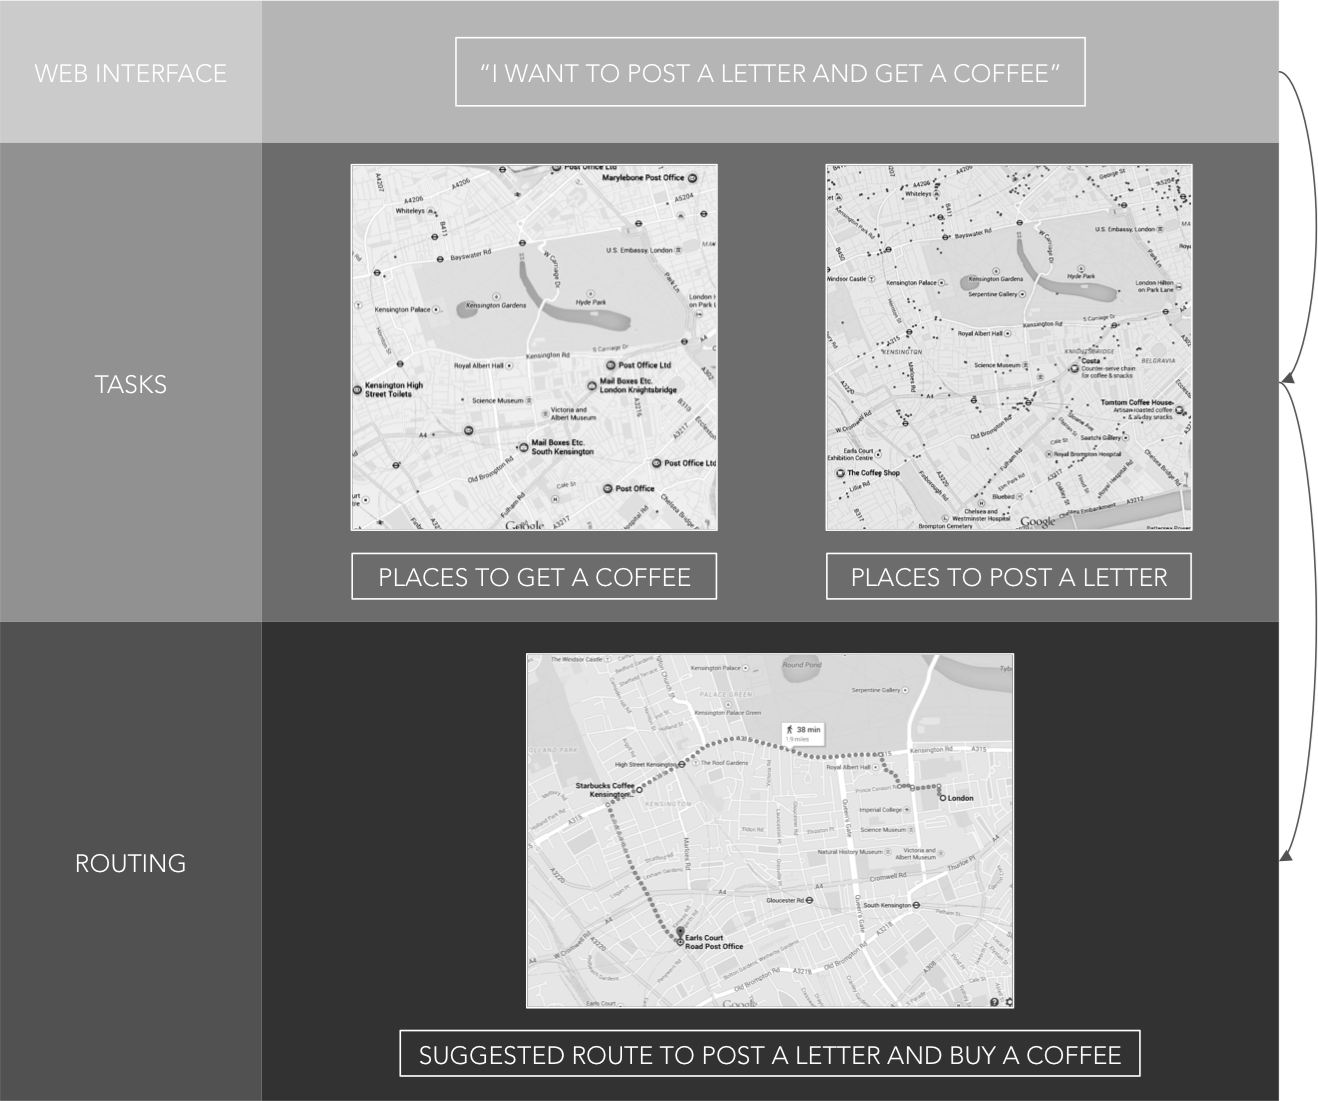
\includegraphics[scale=0.4]{layer_diagram.png}\\
Figure 1. Diagram illustrating the three distinct layers in our application.
\end{center}

\begin{center}
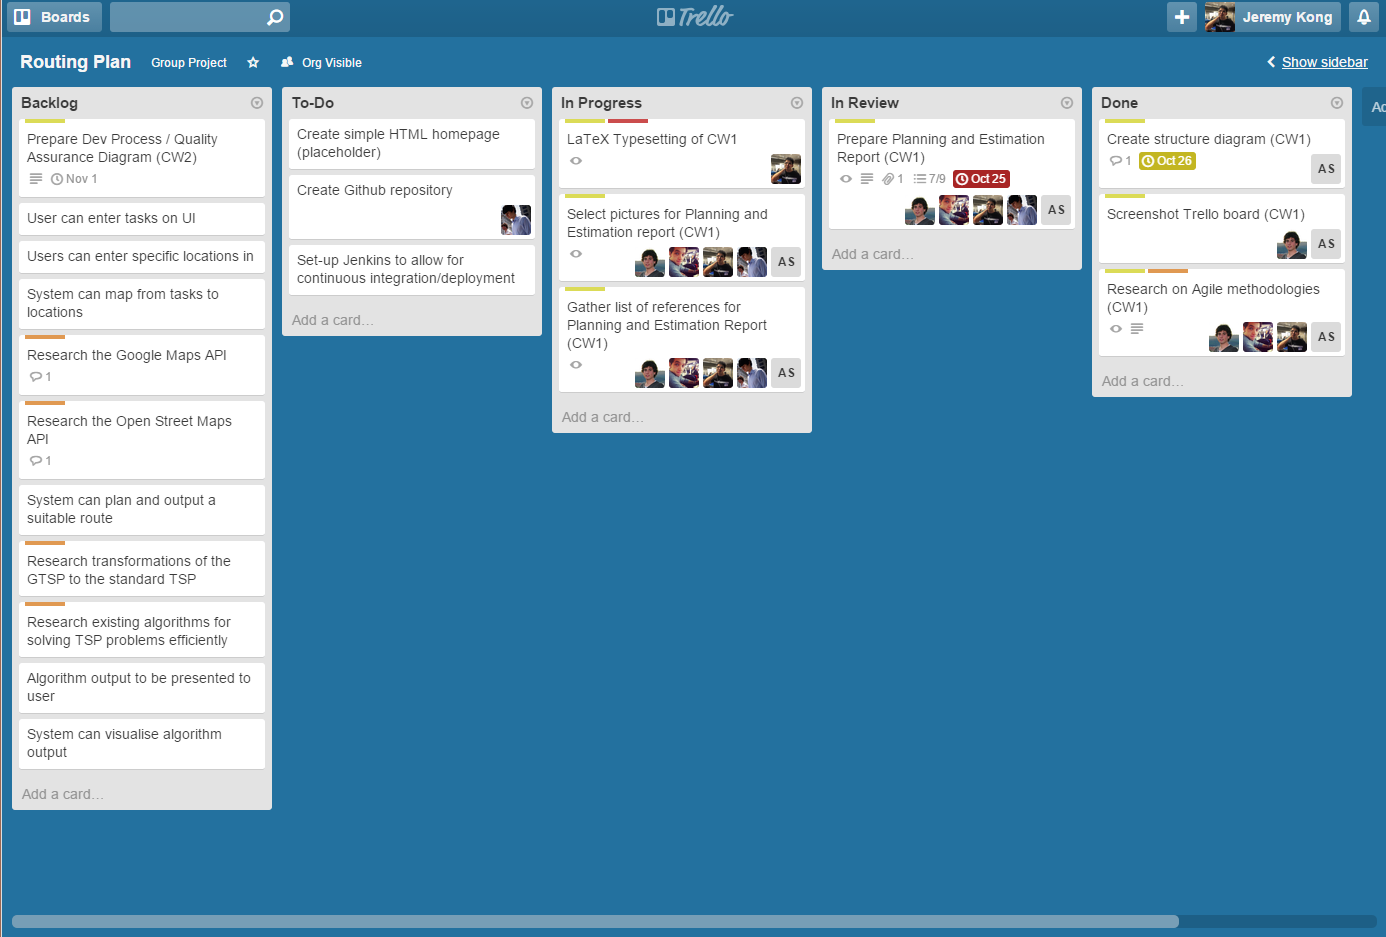
\includegraphics[scale=0.3]{trello_board.png}\\
Figure 2. Screenshot of our Trello board.
\end{center}

\begin{center}
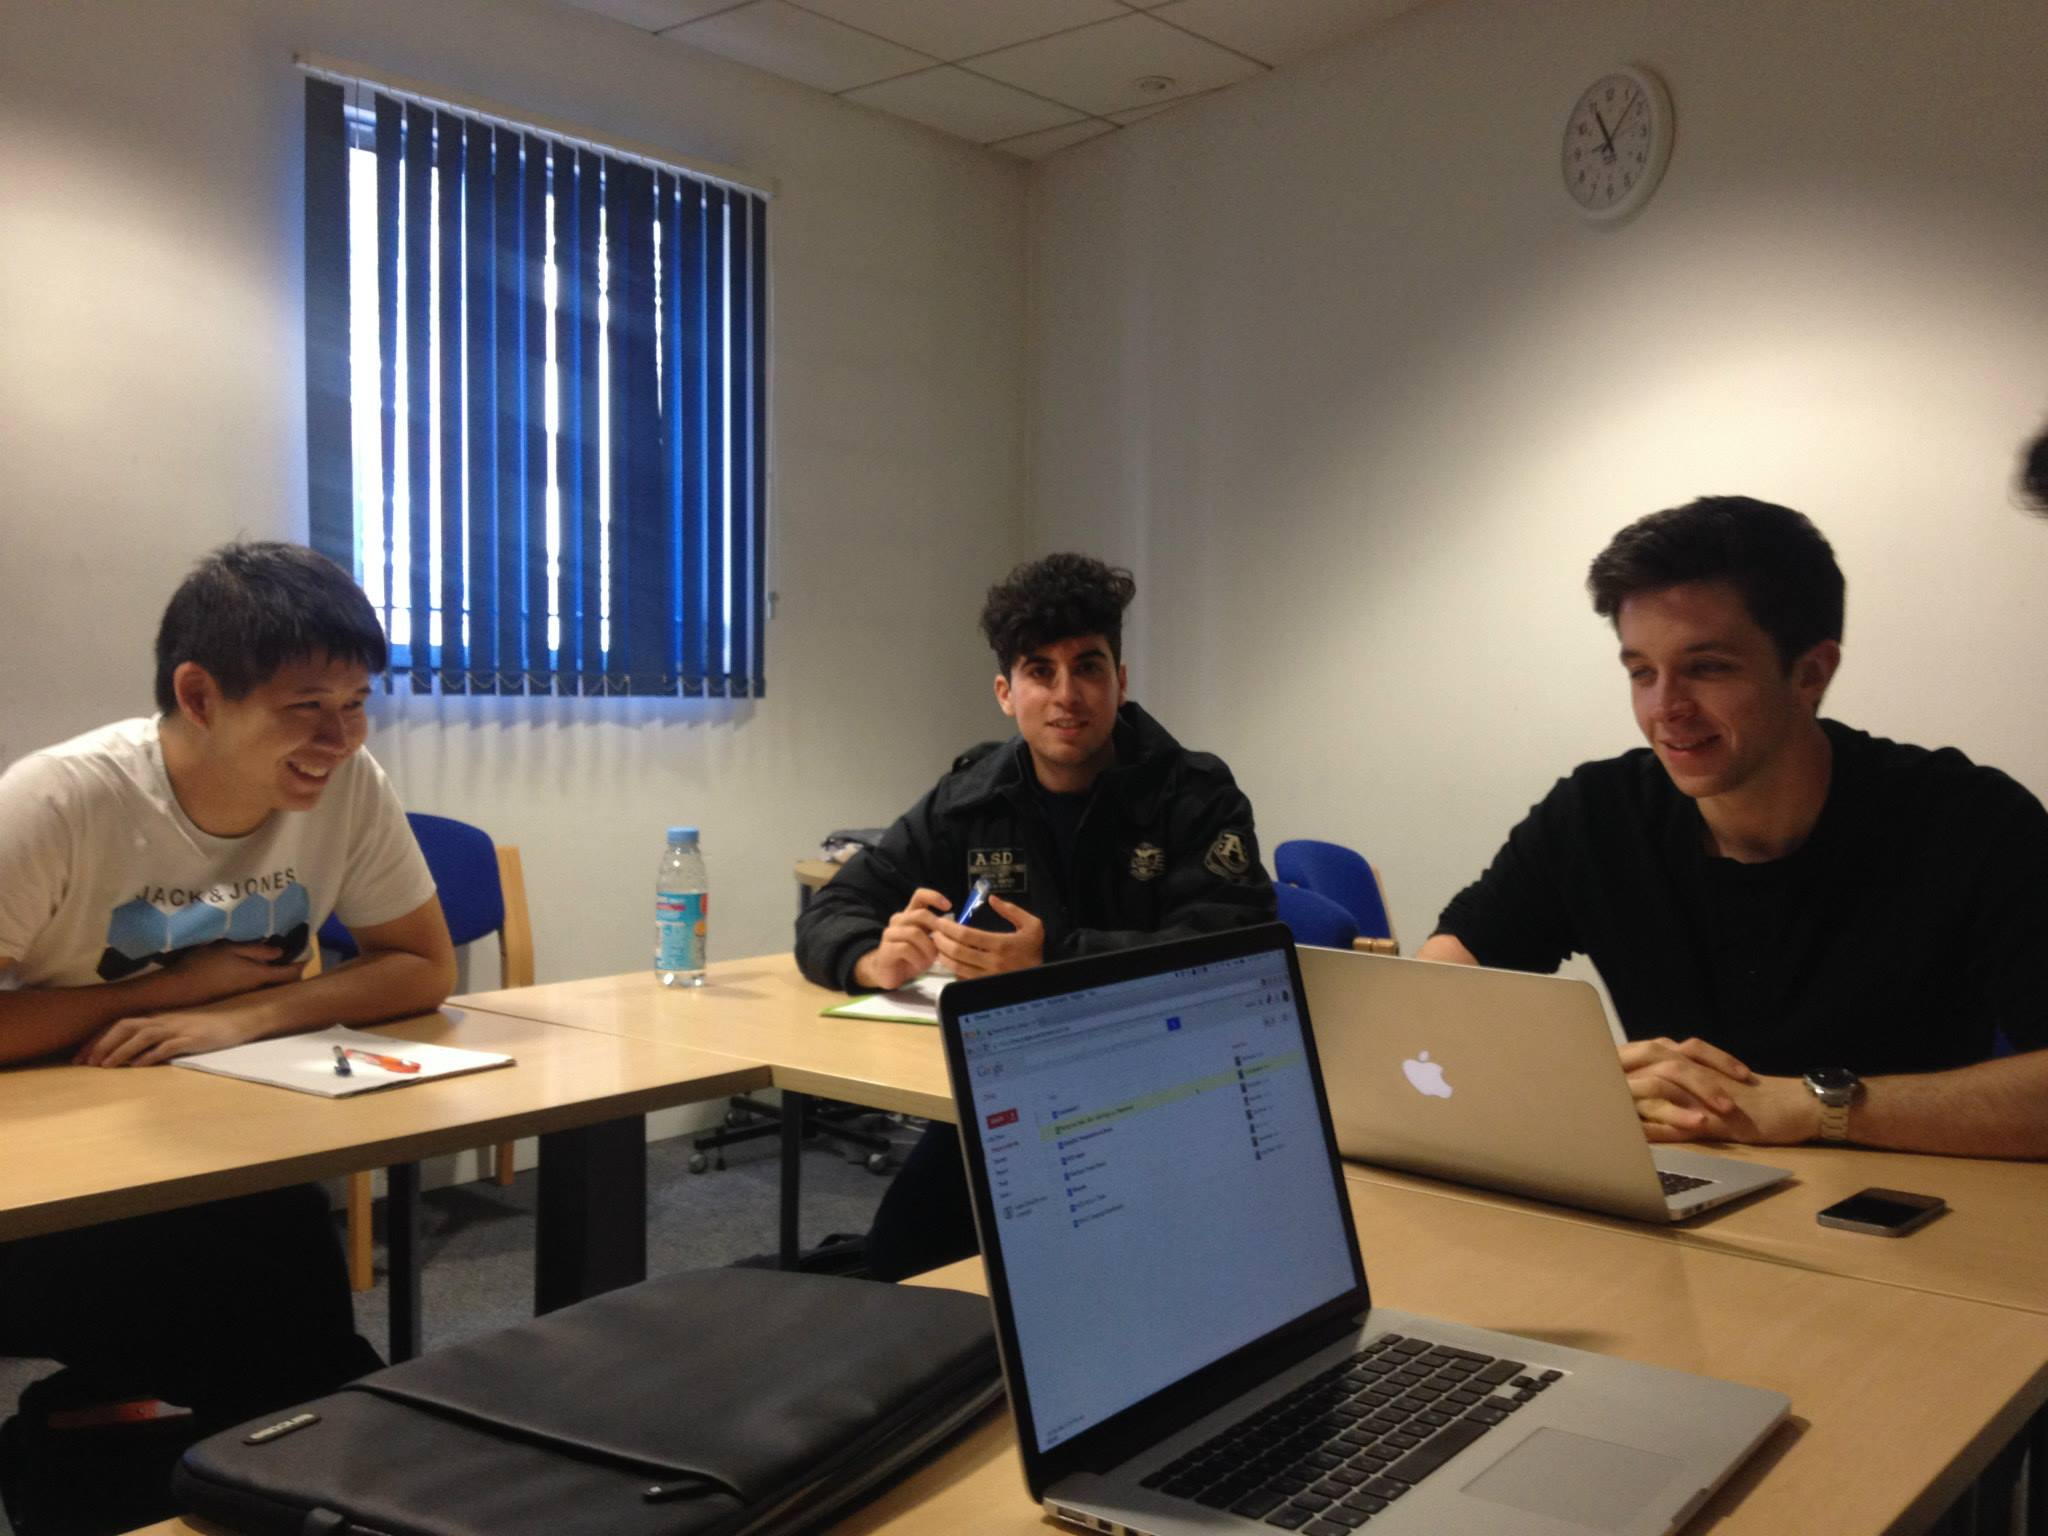
\includegraphics[scale=0.2]{meeting.png}\\
Figure 3. Group brainstorming session.
\end{center}

\begin{center}
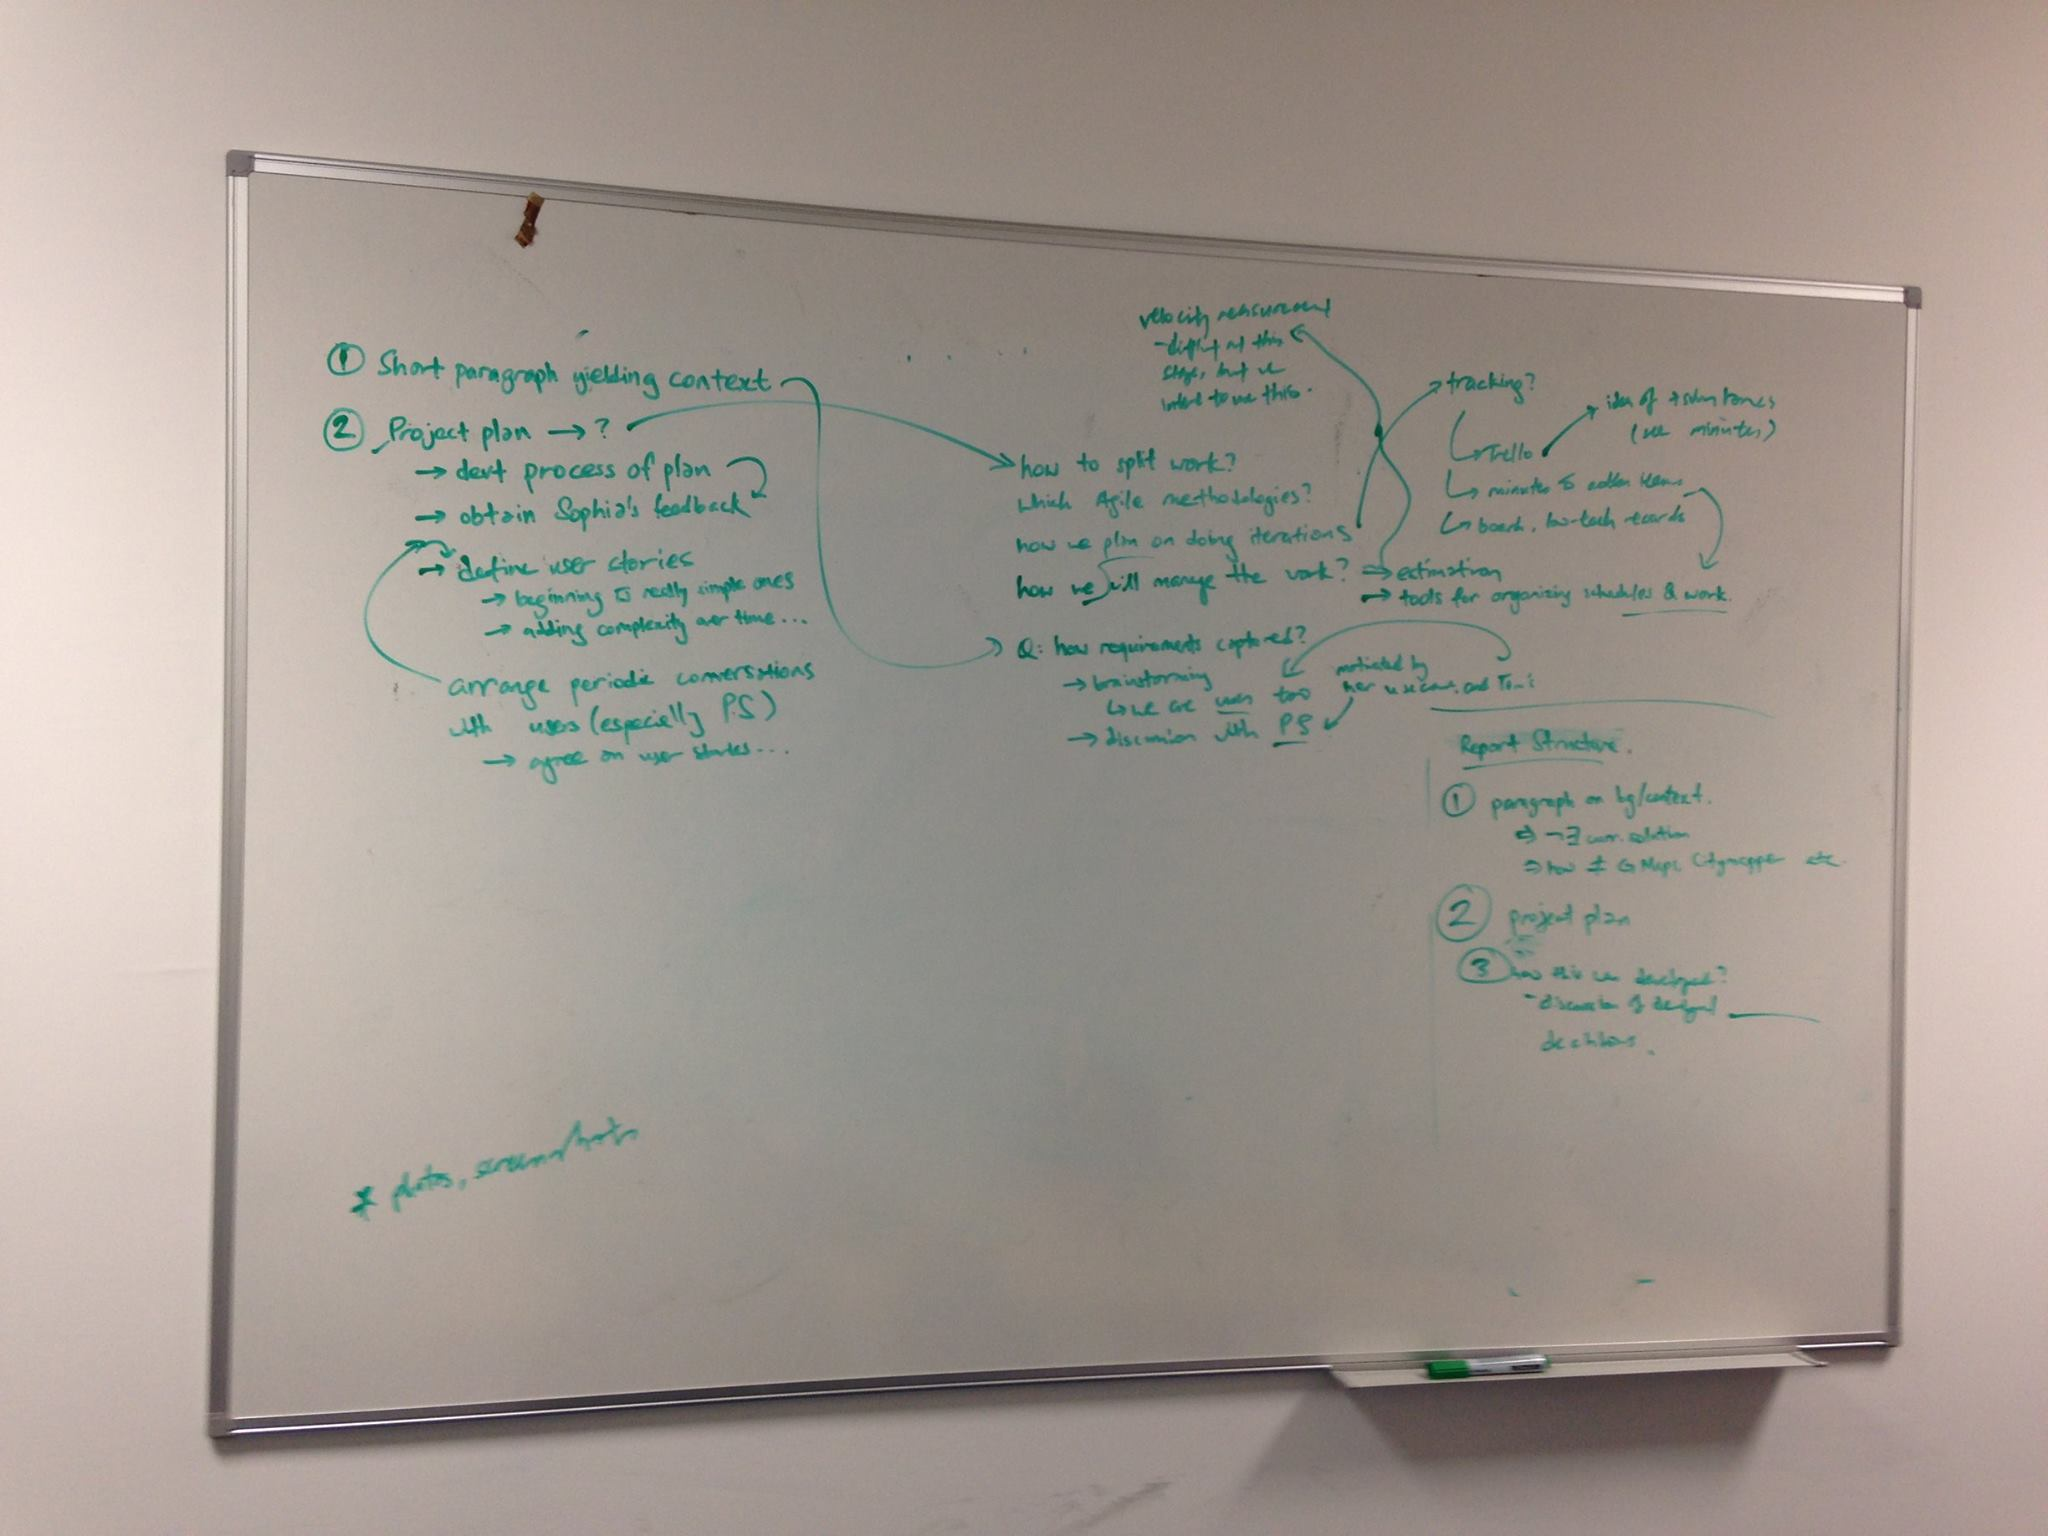
\includegraphics[scale=0.2]{documentation_process.png}\\
Figure 4. Preparation for writing design document.
\end{center}



\end{document}